% !TeX root = RJwrapper.tex
\title{Benchmarking R packages for Calculation of Persistent Homology}
\author{by Eashwar V. Somasundaram, Shael E. Brown, Adam Litzler, Jacob G. Scott, and Raoul R. Wadhwa}

\maketitle

\abstract{%
Several persistent homology software libraries have been implemented in
R. Specifically, the Dionysus, GUDHI, and Ripser libraries have been
wrapped by the \textbf{TDA} and \textbf{TDAstats} CRAN packages. These software represent
powerful analysis tools that are computationally expensive
and, to our knowledge, have not been formally benchmarked. Here, we
analyze runtime and memory growth for the 2 R packages
and the 3 underlying libraries. We find that datasets with less than 3
dimensions can be evaluated with persistent homology fastest by the
GUDHI library in the \textbf{TDA} package. For higher-dimensional datasets, the
Ripser library in the TDAstats package is the fastest. Ripser and \textbf{TDAstats}
are also the most memory-efficient tools to calculate persistent homology.
}

\hypertarget{introduction}{%
\section{Introduction}\label{introduction}}

Topological data analysis (TDA) is a broad set of methodologies that
characterizes structural features of datasets inspired by topological
principles. It has a broad range of usage, from viral evolution to
physical chemistry \citep{TDA-Viral,TDA-PChem}. Within the umbrella of
TDA, persistent homology represents an algebraic approach to
understanding the number, characteristics, and persistence of structural
features in an \(n\)-dimensional point cloud. In the basic workflow of
persistent homology, a series of simplicial complexes are generated on
point clouds to characterize topological features. There are several
methods to generate these complexes on point clouds. In this paper, we
focus on persistent homology of the Vietoris-Rips and alpha complexes,
which use simplicial complexes to approximate topologic relationships in
point clouds. The exact method of constructing these complexes is
described in the Mathematics section. Essentially, we measure features
that are discovered by the algorithm at a particular stage and disappear
at a later stage. The difference between these stages is persistence. Features with larger persistence more likely represent real
geometric patterns rather than noise.

There are several C++ libraries available to researchers that calculate
alpha and Vietoris-Rips complexes, such as Dionysus, GUDHI, and Ripser
\citep{Dionysus,gudhi,Ripser}. These libraries have been wrapped in R by
the \CRANpkg{TDA} and \CRANpkg{TDAstats} packages \citep{TDA,TDAstats}.
Although useful, calculating persistent homology for large datasets is
often limited due to computational complexity \citep{roadmap}. As a
result, researchers often limit persistent homology analysis to lower
dimensions. However, ignoring features in higher dimensions may cause
significant information loss, underutilizing persistent homology's
capabilities. Here, we aim to benchmark two R packages - \CRANpkg{TDA}
and \CRANpkg{TDAstats} - and enable researchers to most efficiently
calculate persistent homology in R.

\hypertarget{mathematics-of-persistent-homology}{%
\section{Mathematics of Persistent
Homology}\label{mathematics-of-persistent-homology}}

An \(n\)-dimensional simplex is the convex hull of \(n+1\) points in a
Euclidean space. More intuitively, an \(n\)-dimensional simplex is the
simplest \(n\)-dimensional object (e.g.,~a 0-simplex is a point, a
1-simplex is a line, a 2-simplex is a triangle, 3-simplex is a
tetrahedron). These simplices can be glued together on common
sub-simplices to form a simplicial complex (e.g.,~two triangles sharing a
common side). In a simplicial complex, topological features will arise
that can be characterized by Betti numbers. Each Betti number, denoted
by \(B_k\), \(k\) counts the number of features in dimension \(k\).
\(B_0\) counts the number of connected components, \(B_1\) counts refer
to loops, \(B_2\) counts the number of voids, and so on
\citep{phom-survey}.

There are several different methods to construct a simplicial complex on
a given point cloud \(S\), but this paper focuses on the Vietoris-Rips
and alpha complexes. The Vietoris-Rips complex is perhaps the most
common method for constructing a simplicial complex to calculate
persistent homology \citep{Rips-Complex}. In a point cloud of \(k\)
points in 2 dimensions, a distance parameter, \(\delta > 0\), can be
used to draw a circle of diameter \(\delta\) around every point in
\(S\). For point clouds in 3 dimensions, spheres of diameter \(\delta\)
are drawn around each point. For dimensions \(k\) greater than 3, a
\(k\)-dimensional hypersphere is drawn around each point. The remainder
of this explanation will focus on the 2-dimensional case. If \(\delta\)
is sufficiently large, then some of the resulting circles may intersect.
In this case, a line is drawn to connect the points at the center of the
intersecting circles. When a triple of points is connected, we add a
triangle (2-simplex). When a quadruple of points are connected, we add a
tetrahedron (3-simplex) and so forth. However, we only add simplices at
most of the dimension of the space of the point clouds (e.g.,~only up to
3-simplices are added in a 3-dimensional point cloud). This group of
points and lines form the skeleton of a simplicial complex. For each
distance parameter, \(\delta\), there will be a single simplicial
complex associated with it. As \(\delta\) increases, different
topological features may appear, persist, and eventually disappear.

Once \(\delta\) reaches the maximum Euclidean distance between any pair
of points in the point cloud, a convex hull will form around all \(k\)
points creating a \((k-1)\)-dimensional simplex. A 3-column matrix can
be created recording the dimension of each feature, the \(\delta\) at
which that feature appeared, and the \(\delta\) at which it disappeared.
This matrix characterizes the persistent homology of that point cloud.

\begin{figure}
  \centering
  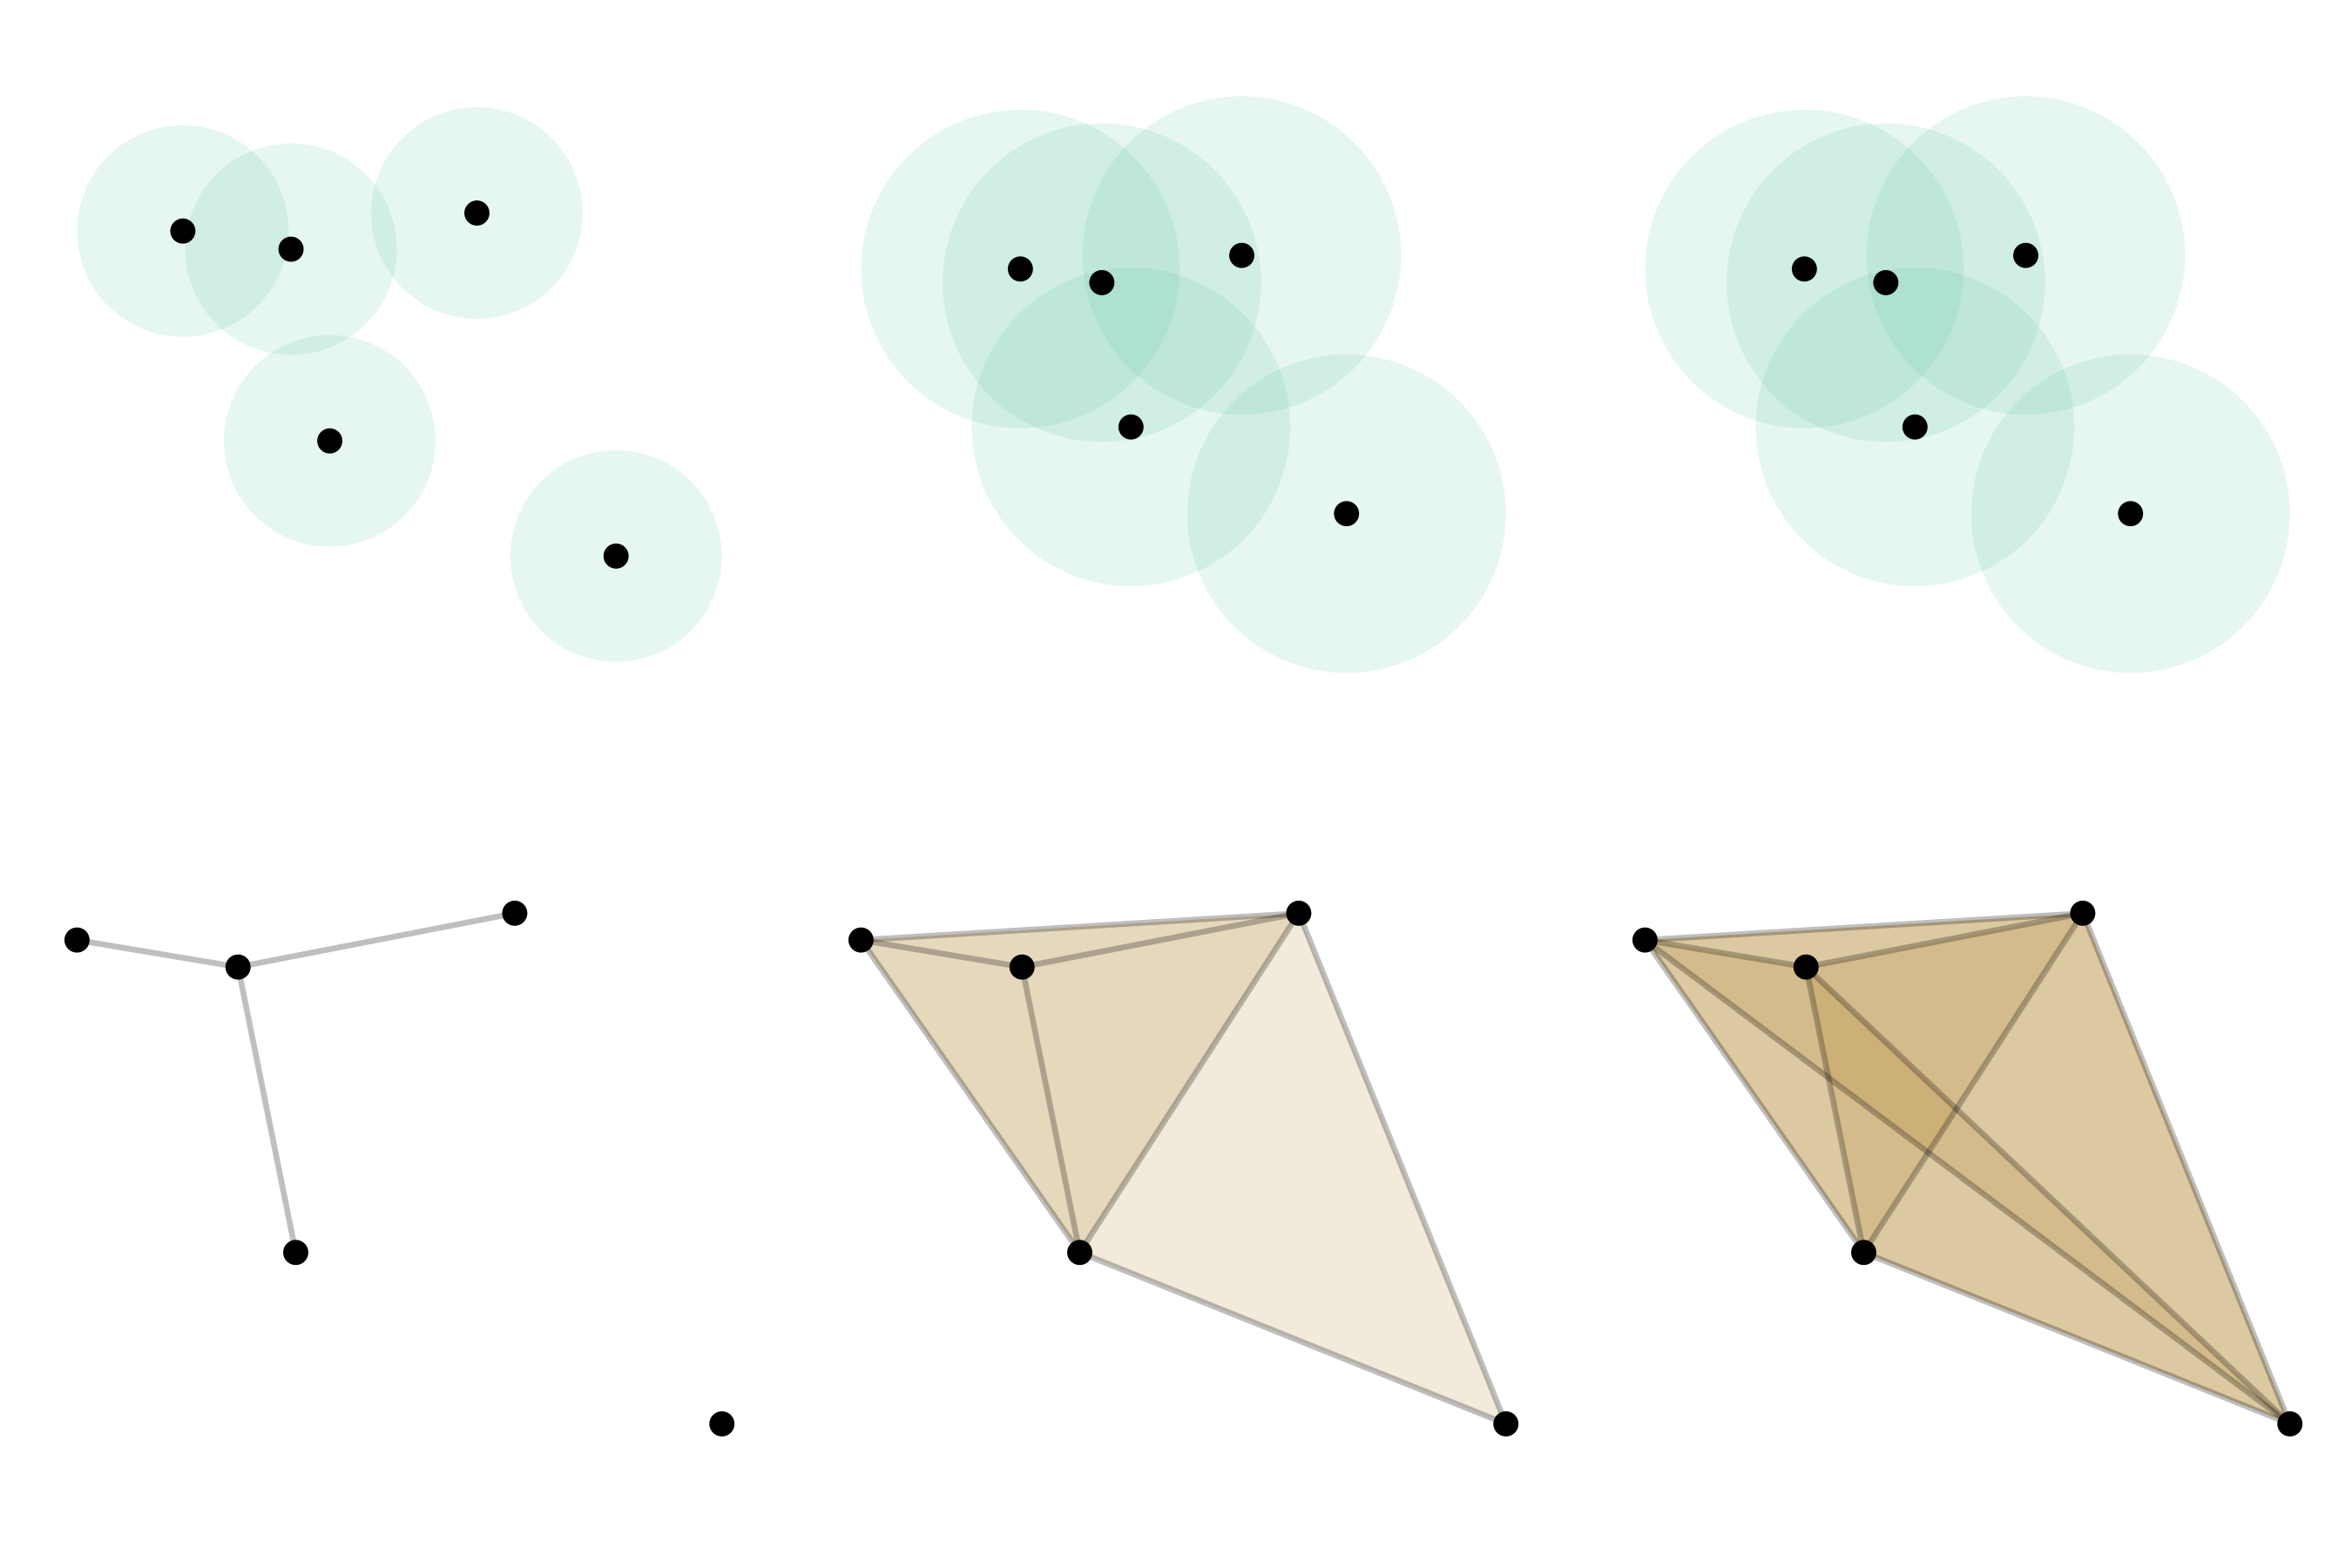
\includegraphics[height=2.5in]{fig1.png}
  \caption{\textbf{Basic Visualization of the Vietoris-Rips Complex.}
  For a given parameter, $\delta$, $\delta$-diameter circles are drawn around each point.
  If two circles intersect, a point is drawn between their centers.
  As $\delta$ continues to grow, more circles intersect, filling out the simplicial complex.
  Features on the simplicial complex appear and die as $\delta$ increases.
  These features' dimensions, birth, and death are recorded in an $n$x3 matrix.
  Eventually, the full convex hull is drawn, ending the "filtration" process.}
\end{figure}

Alpha complexes provide another method to generate simplicial complexes
on the point cloud \(S\). For alpha complexes, we partition the whole
space in which the data resides into cells such that each cell contains
exactly one data point \(x\), and the cell of that data point is the set
of all points closer to \(x\) than any other data points. Such a
partition is also known as a Voronoi diagram. The nerve of a Voronoi
diagram is equivalent to the Delaunay Triangulation
\citep{alpha-complex}. Alpha complexes are simplicial complexes that are
subsets of the Delaunay Triangulation. The parameter, \(\alpha\), can
describe the radius of a ball (dimension matches dimension of the space)
of each point in the point cloud \(S\) much, like \(\delta\) describes
the diameter of a circle in the Vietoris-Rips complex. We first
intersect the \(\alpha\) radius balls with their own Voronoi cell and
then search for intersections of these subsetted balls to form
simplices. Once \(\alpha\) is large enough, the full Delaunay
Triangulation is formed. In between these stages, the birth and death of
features at certain values of \(\alpha\) can be captured in a 3-column
persistent homology matrix much like the Vietoris-Rips complex. One key
difference from the Vietoris-Rips complex is that edges can only form
between neighboring points in the alpha complex.

\begin{figure}[b]
  \centering
  \includegraphics[width=4in]{fig2.png}
  \caption{\textbf{Basic visualization of the Alpha complex.}
  For a given $\alpha$, $\alpha$-radius balls are drawn around each point, and the union of the balls is taken.
  Then, an intersection between this union of $\alpha$-balls and the Vornoi diagram is taken.
  A connecting segment is drawn between points in adjacent Voronoi cells once the $\alpha$-ball fills out the Voronoi diagram.
  As $\alpha$ grows, more circles fill out the Voronoi cells.
  Once $\alpha$ is large enough, the Delaunay Triangulation is formed.}
\end{figure}

In both methods, the boundary matrix records all simplicial complexes
for each parameter value (\(\delta\) for Vietoris-Rips complexes and
\(\alpha\) for alpha complexes). Calculating persistent homology is
divided into two steps: (1) forming the boundary matrix and (2)
reducing the boundary matrix to be able to read off the topological
features of each dimension and their birth/death values of the
parameter. The second step can be computed in at most O(k\^{}3) steps,
where k is the number of rows (and columns) of the boundary matrix. The
size of the boundary matrix can describe the memory complexity on the
random access memory (RAM) for persistent homology calculations. We
compare memory complexity between alpha and Vietoris-Rips complexes in
this paper.

Alpha complex calculations have a run time complexity of \(O(n^{d/2})\),
and Vietoris-Rips complex calculations have a run time complexity of
\(O(2^n)\), where \(n\) is the number of points and \(d\) is the point
cloud dimension \citep{roadmap}. Vietoris-Rips's run time and memory are
exponential with regards to point number (but constant with data
dimension) in contrast to alpha complexes where run time and memory are
polynomial with point number (but exponential with data dimension).
Therefore, we can predict that low dimensional point clouds favor alpha
complexes, but fewer points in higher dimension favor Vietoris-Rips
complexes.

\begin{figure}[tb]
  \centering
  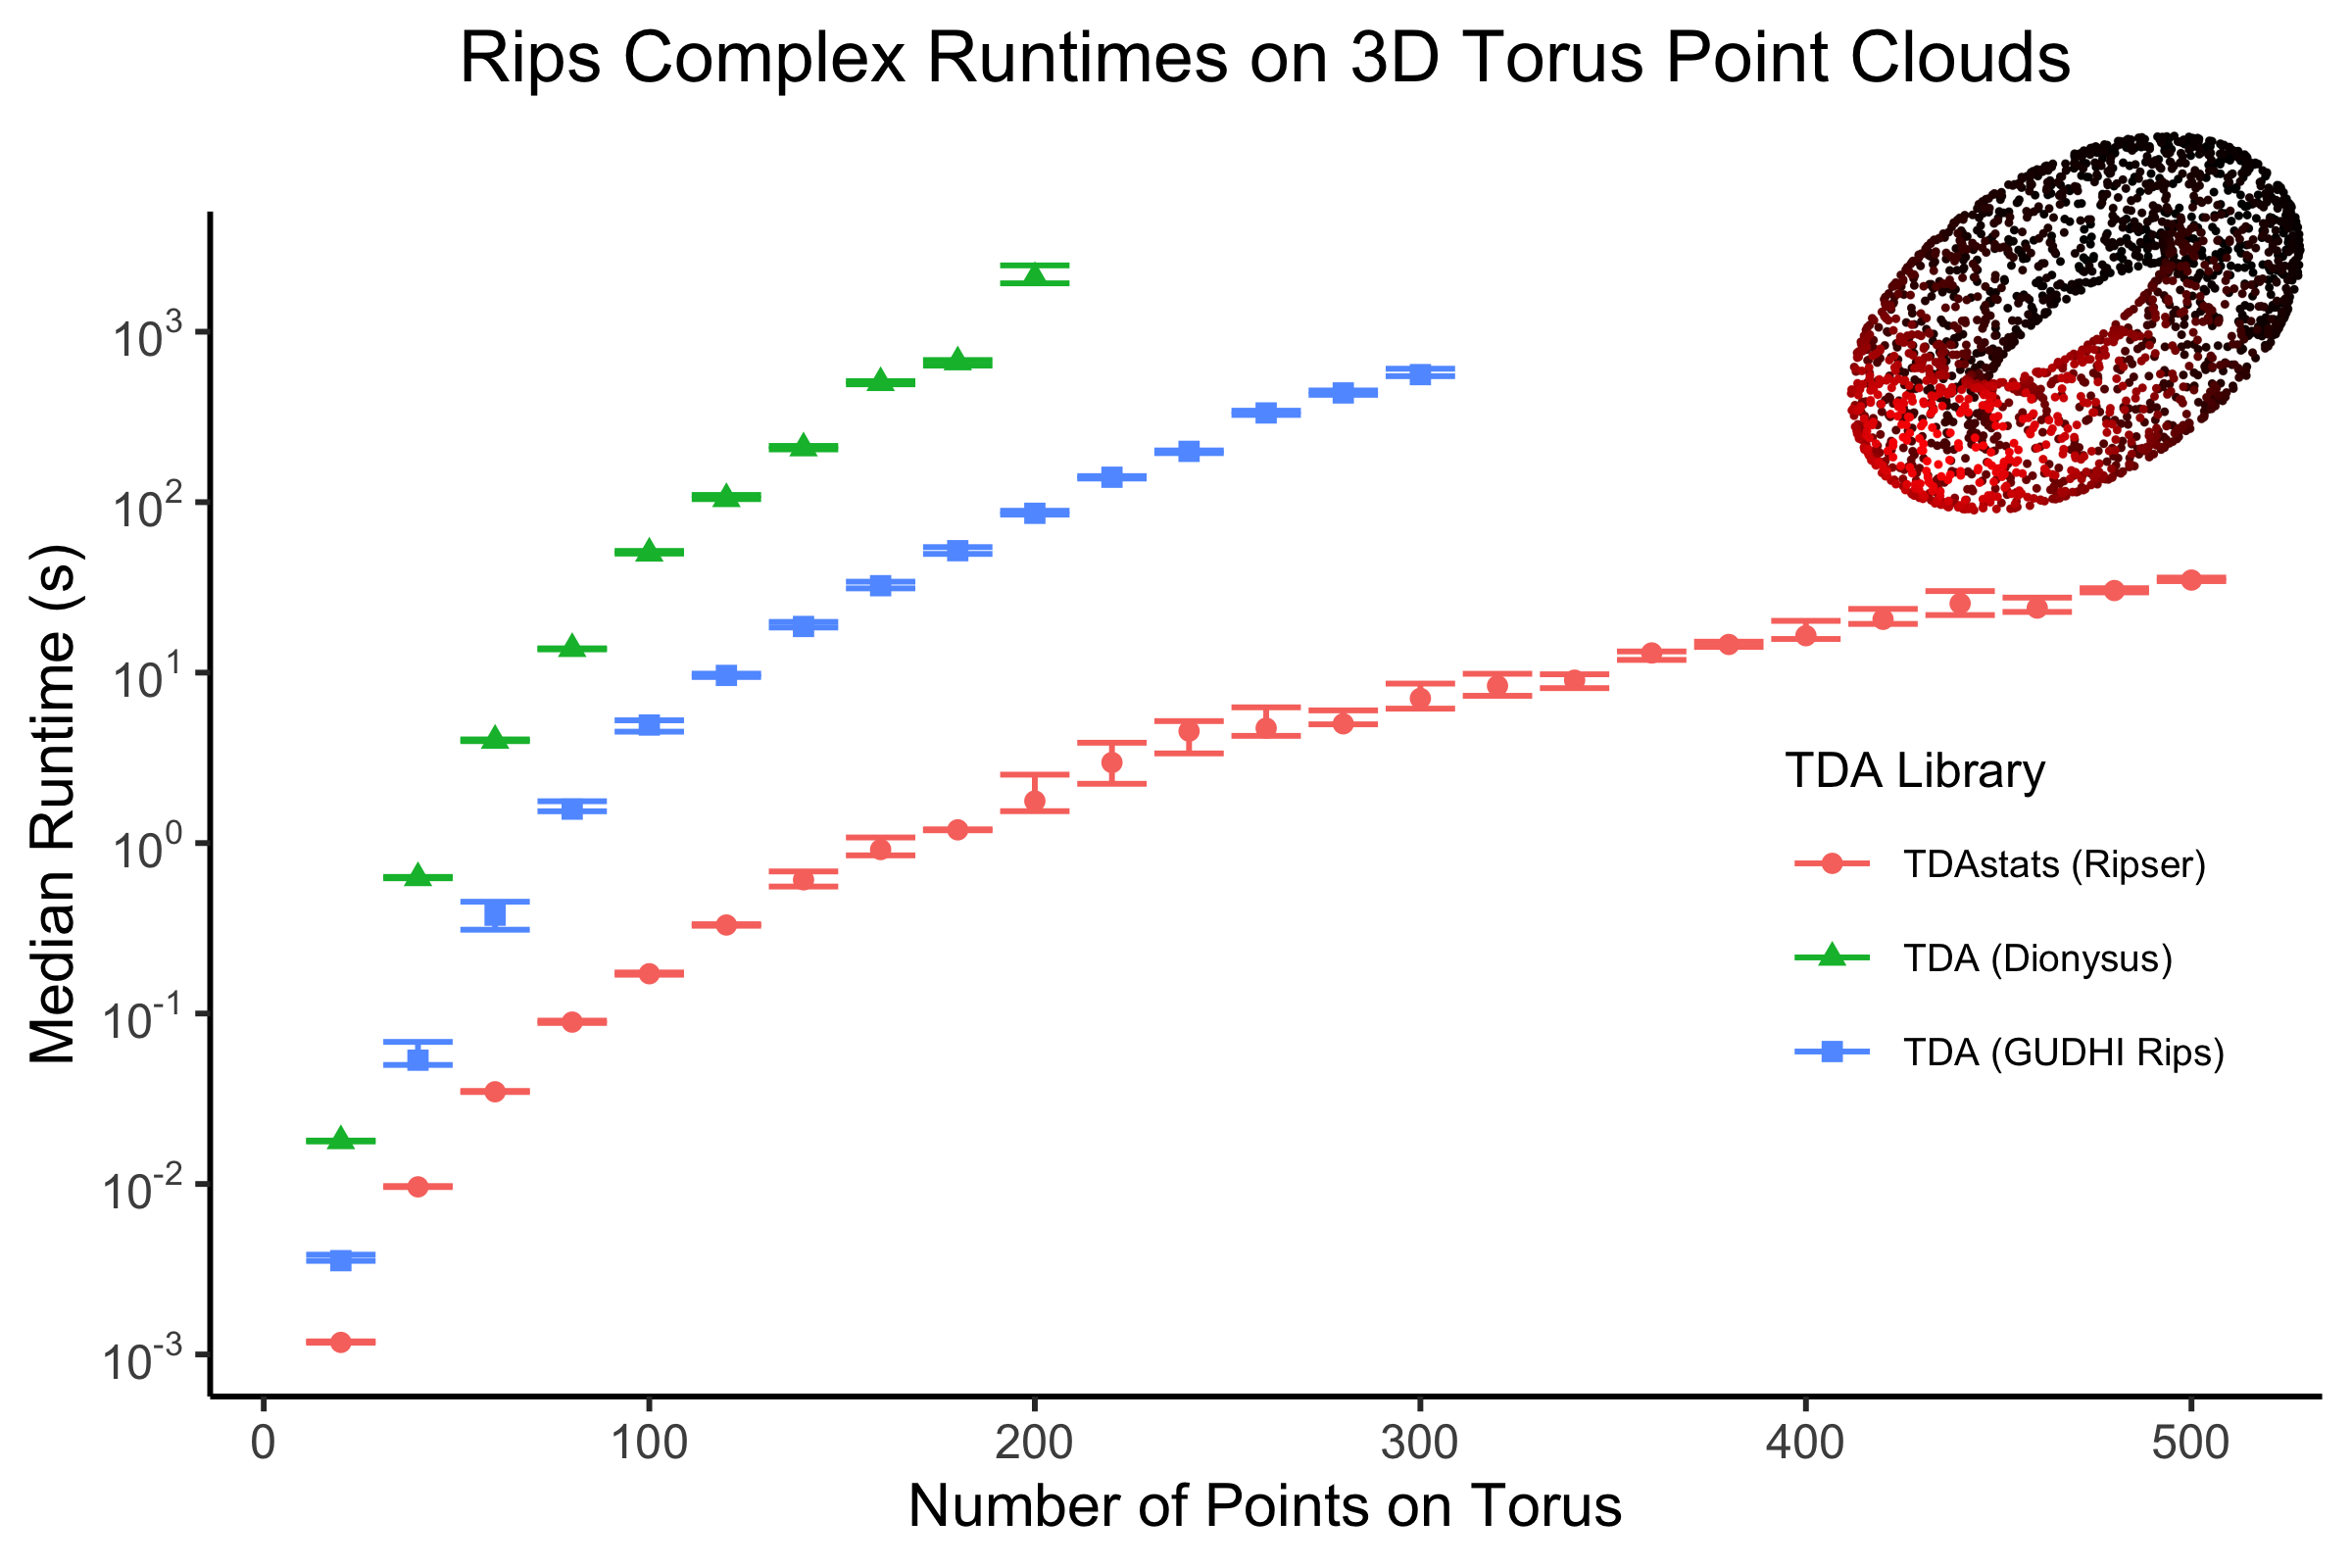
\includegraphics[height=2.5in]{fig3.png}
  \caption{
    \textbf{Calculating persistent homology of a torus with three TDA libraries.}
    Median runtime (min to max, $n=10$ iterations per data point) for each TDA library (denoted by color) is plotted against point cloud size.
    Homological features of up to 2 dimensions were calculated.
    Time complexity follows a power law for all three libraries (see GitHub repo for regression details).
    Although the libraries have similar runtimes for smaller point clouds, Dionysus has a clear disadvantage when the number of points exceeds 100.
    When the number of points exceeds 200, Ripser has a clear advantage over GUDHI, which maintains its advantage over Dionysus.
  }
\label{fig:tor}
\end{figure}

\hypertarget{methods}{%
\section{Methods}\label{methods}}

We use \CRANpkg{readr} v1.3.1 to read rectangular data \citep{readr},
\CRANpkg{ggplot2} v3.2.1 \citep{ggplot2}, \CRANpkg{scatterplot3d}
v0.3-41 \citep{scatterplot3d}, \CRANpkg{recexcavAAR} v0.3.0
\citep{recexcavAAR}, \CRANpkg{deldir} v0.1 \citep{deldir}, ggtda v0.1
\citep{ggtda}, and \CRANpkg{magick} v2.2 \citep{magick} to visualize
data, \CRANpkg{bench} v1.0.4 to collect benchmark data \citep{bench},
\CRANpkg{TDA} v1.6.9 \citep{TDA} and \CRANpkg{TDAstats} v0.4.1
\citep{TDAstats} to calculate persistent homology of Vietoris-Rips and
alpha simplicial complices, and \CRANpkg{pryr} v0.1.4 for calculations
involving R objects \citep{pryr}. Median runtime calculations are shown
along with the minimum and maximum of 10 iterations per benchmark.
Datasets were generated by sampling functions in base R to generate
points uniformly distributed over circles (dimension = 2), spheres
(dimension = 3), filled squares (dimension = 2), filled cubes (dimension
= 3, 4), and tori (dimension = 3). The number of points per point cloud
varied from 25 to 500 along with intervals of 25 points, which were empirical
limits chosen after considering available computational resources. For
consistency between software libraries, the minimum and maximum
simplicial complex radii were predetermined for each point cloud and
provided as parameters to the \CRANpkg{TDA} and \CRANpkg{TDAstats} R
packages. Within the \CRANpkg{TDA} package, benchmark data was collected
for the GUDHI \citep{gudhi} and Dionysus \citep{Dionysus} libraries;
within the \CRANpkg{TDAstats} package, benchmark data was collected for
the Ripser \citep{Ripser} library. As alpha complex calculation was only
implemented in GUDHI, alpha complex benchmark data was naturally only
collected for the single library. Measuring memory usage proved
challenging since all the libraries calculating persistent homology were
implemented in either C++ or Java and then wrapped in R as part of a
CRAN package. Thus, memory burden was indirectly measured by using
boundary matrix size as a proxy. Given that Ripser optimizes computation
of persistent homology by avoiding calculation of a boundary matrix,
memory use benchmarks are not provided for Ripser and, consequently,
\CRANpkg{TDAstats}.

Benchmark data were collected twice - once on a local machine and once on
a remote computing node, each of which featured 16 GB RAM. Both datasets
were compared for consistency and are publicly available at the
repository linked below. Data from the remote computing node is
visualized in this report. The larger point clouds required more than 16
GB of RAM to calculate persistent homology using a subset of the
libraries; attempts to compute results resulted in runtime errors, and
the corresponding output is missing from the corresponding figures and
tables. Fully reproducible code for all numerical results and figures
can be found at \url{https://github.com/eashwarsoma/TDA-benchmark}. This
GitHub repository also contains instructions for generating the
Supplement referenced in this report's results. Video explanations of
TDA concepts and reproducing all results in this report can be found at
\url{https://tinyurl.com/TDABench}.

\begin{widefigure}[bt]
  \centering
  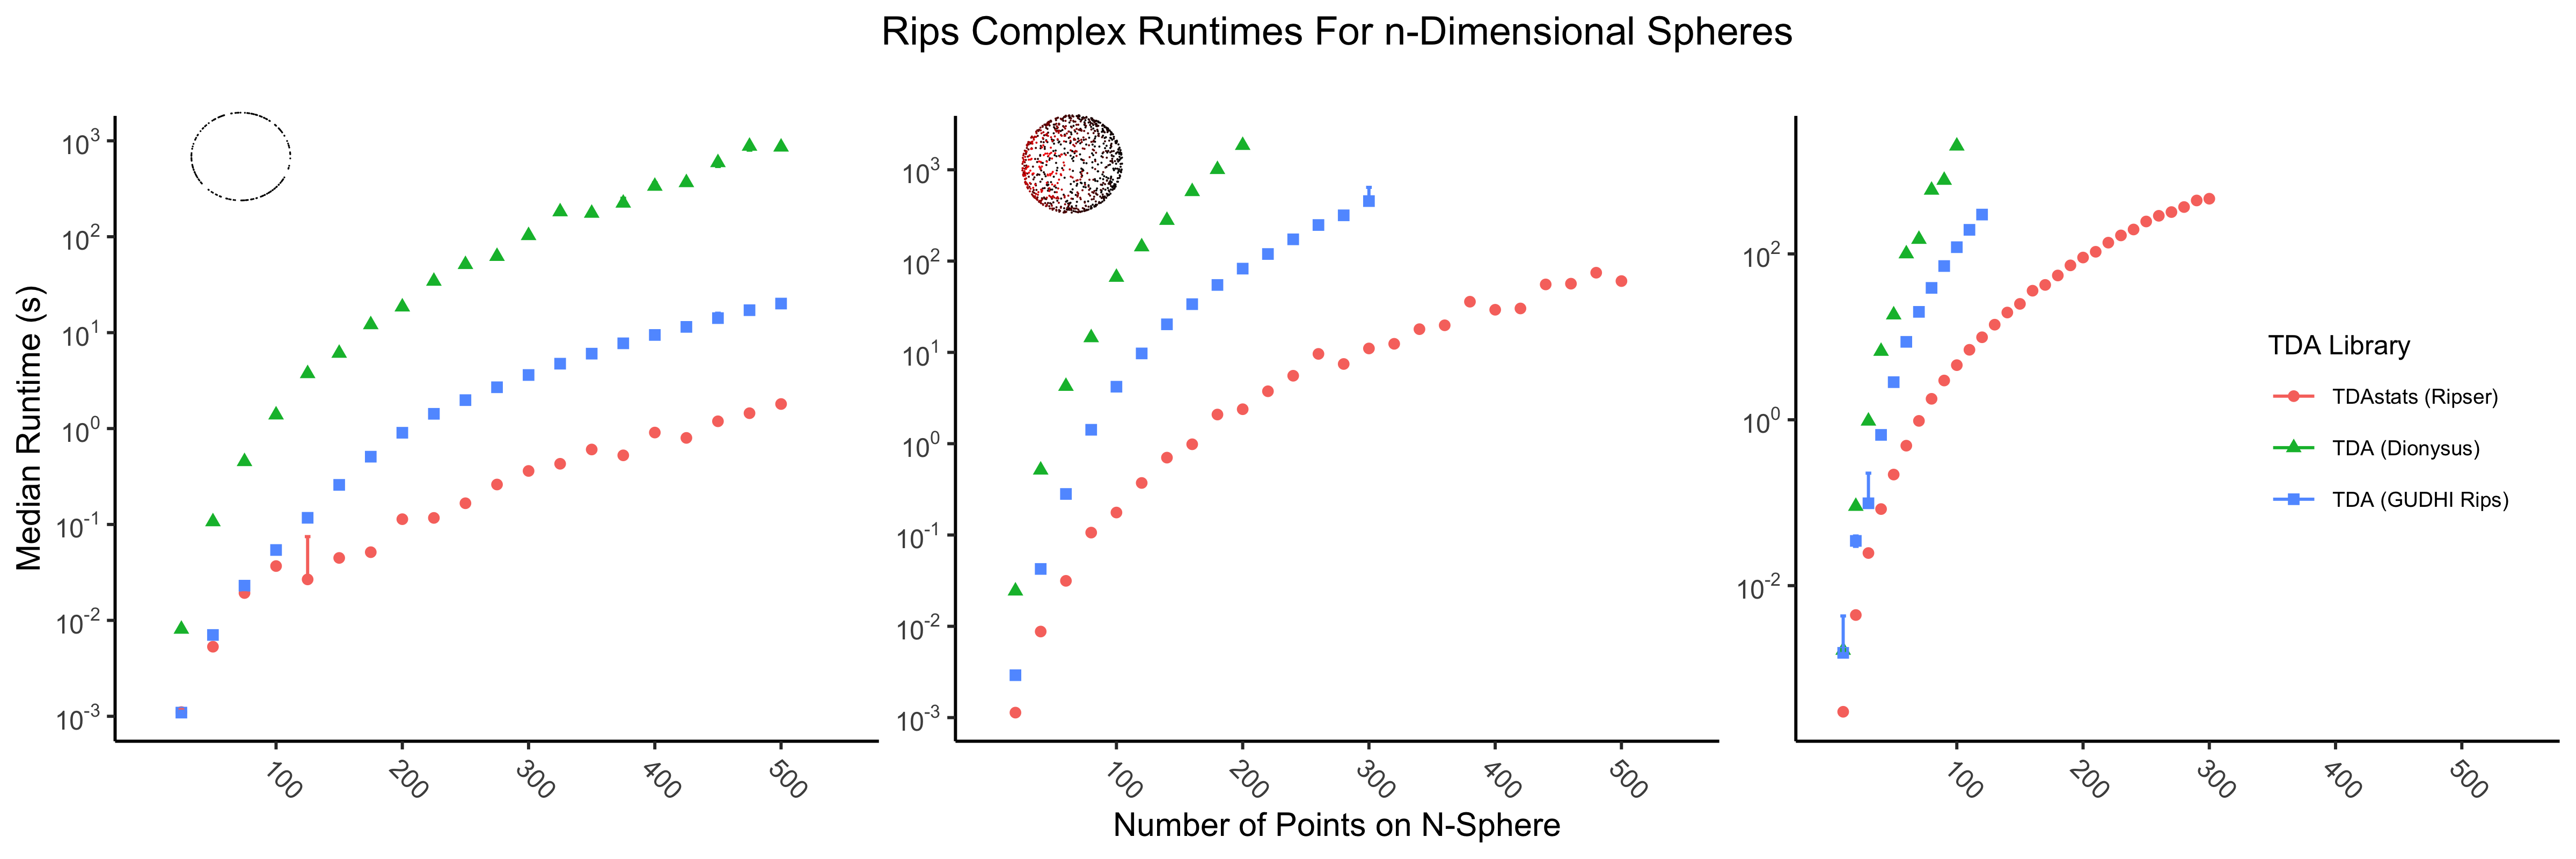
\includegraphics[height=2in]{fig4.png}
  \caption{
    \textbf{Calculating persistent homology of round point clouds of varying dimensions with three TDA libraries.}
    Median runtime (min to max, $n=10$ iterations per data point) for each TDA library (denoted by color) is plotted against point cloud size and faceted by data dimension.
    The left panel compares library performance for a 2-dimensional circular point cloud, the center panel for a 3-dimensional spherical point cloud, and the right panel for a 4-dimensional hyperspherical point cloud.
    Maximum feature dimensions (one less than the data dimension) were calculated in each case.
  }
\label{fig:cir}
\end{widefigure}

\hypertarget{results}{%
\section{Results}\label{results}}

Computing persistent homology of a canonical torus grants quick insight
into efficiency of each library (Figure \ref{fig:tor}). Dionysus
exhibits the longest median runtime, and, although Ripser and GUDHI have
similar runtimes for smaller point clouds, as the number of points
increases Ripser eventually has a significant lead. Next, we compare
library performance with multiple canonical datasets to ensure that the
noted pattern generalizes.

\begin{widefigure}
  \centering
  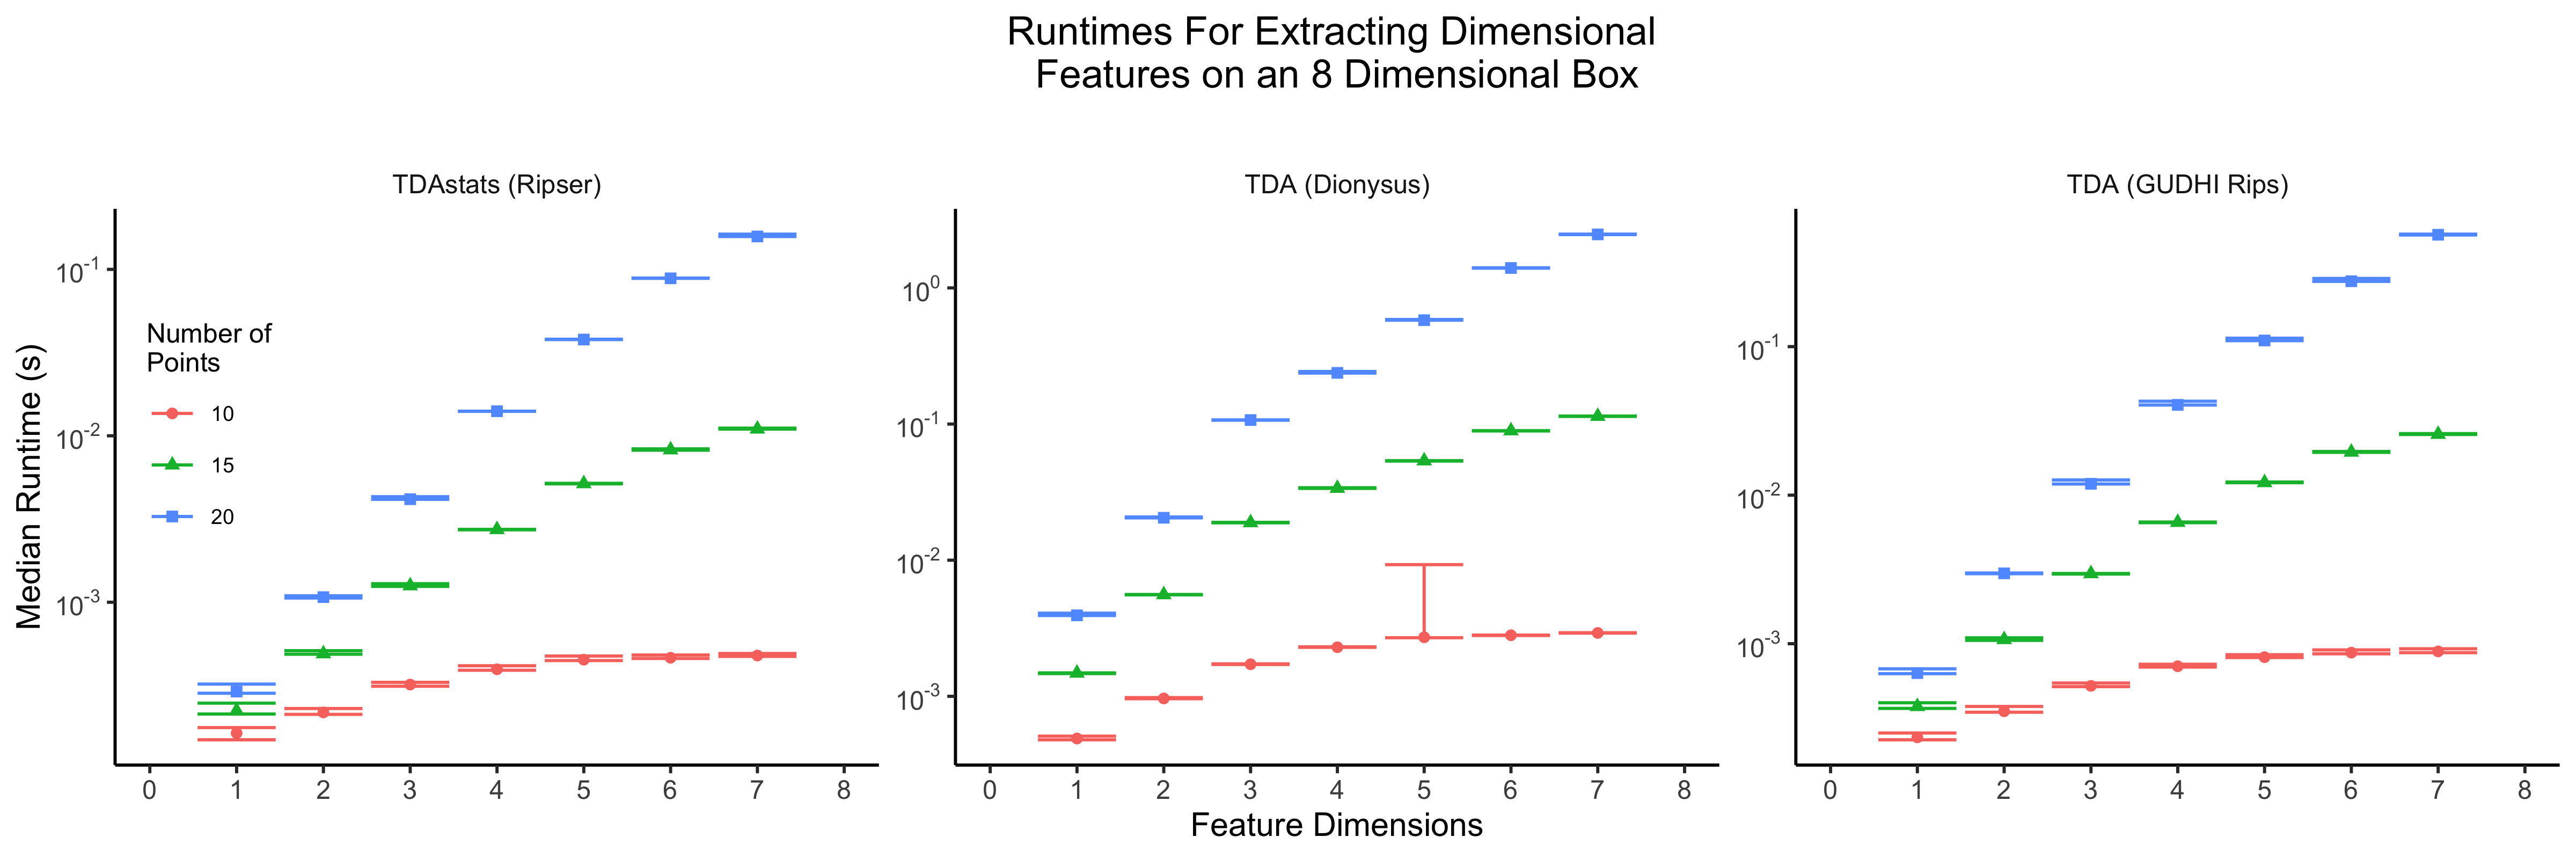
\includegraphics[height=2in]{fig5.png}
  \caption{
    \textbf{Comparison of Vietoris-Rips complex persistent homology calculation as a function of feature dimension.}
    Median runtime (min to max, $n=10$ iterations per data point) for various point cloud sizes (denoted by color) is plotted against the calculated feature dimension and faceted by TDA library.
    Persistent homology was calculated on a uniformly distributed random sample of points contained within a 1 unit, 8-dimensional cube.
    Computational limitations of calculating persistent homology for a large number of feature dimensions restricted point clouds to relatively small sizes.}
\label{fig:box}
\end{widefigure}

Tori do not trivially generalize to other dimensions, but circles do.
Benchmarking on a circular point cloud permits confirmation of the
pattern in Figure \ref{fig:tor} while also revealing how the libraries
compare as the dataset dimension increases. Figure \ref{fig:cir} exhibits
the resulting data for a 2-dimensional circle (left panel),
3-dimensional sphere (center panel), and 4-dimensional hypersphere
(right panel). When the dataset dimension equals 2, GUDHI practically
matches Ripser's performance in outpacing Dionysus. However, in the case
of the 3-dimensional sphere, the pattern visualized in Figure
\ref{fig:tor} for the 3-dimensional torus is again present. By the 4th
dimension, the gap between Ripser and GUDHI widens. Of note, missing
points for larger datasets in Figure \ref{fig:cir} are not plotted if
and only if calculating persistent homology caused an error due to
insufficient RAM. Thus, for the hypersphere, Ripser was able to
calculate persistent homology for a dataset with approximately 3 times
as many points as Dionysus and over 2 times as many as GUDHI.
Interestingly, all curves plotted in Figure \ref{fig:cir} grow
polynomially with respect to the number of points (see Supplement for
regression details).

Large data and feature dimensionality often restrict persistent
homology calculations to small point clouds due to computational limits.
When calculating persistent homology on a high-dimensional point cloud,
as Vietoris-Rips feature dimension increases, there is a corresponding
increase in runtime (Figure \ref{fig:box}). Dionysus is clearly
outmatched by GUDHI and Ripser as feature dimension increases, with the
difference being clearest for larger point clouds; by feature dimension
5, Ripser outpaces GUDHI as well (Figure \ref{fig:box}). It is unclear
whether runtime for each library grows polynomially or exponentially
(see Supplement for regression details).

Even with a constant feature dimension, the underlying data dimension
could play a role in the runtime of persistent homology calculation. Figure
\ref{fig:ann} compares the handling of this issue by the Vietoris-Rips
complex and the alpha complex. Since GUDHI is the only library
implementing functionality with an alpha complex, we compare its
implementations of the Vietoris-Rips and alpha complices. Due to
computational limitations, an alpha complex could not be calculated for
any point clouds with data dimensions exceeding 3. Two notable aspects of
Figure \ref{fig:ann} stand out. First, the alpha complex calculation
clearly runs faster than the Vietoris-Rips complex calculation, a trend
that becomes clearer as point cloud size increases. Second, although the
Vietoris-Rips complex calculation runtime appears to be independent of the underlying data dimension, the alpha complex calculation is dependent on it.
Figure \ref{fig:ann} shows a subtle difference between data dimensions 2
and 3 as point cloud size increases. Although unconcerning for a data
dimension up to 3, failure to run any alpha complex calculations with a
data dimension of 4 could be cause for concern.

\begin{figure}
  \centering
  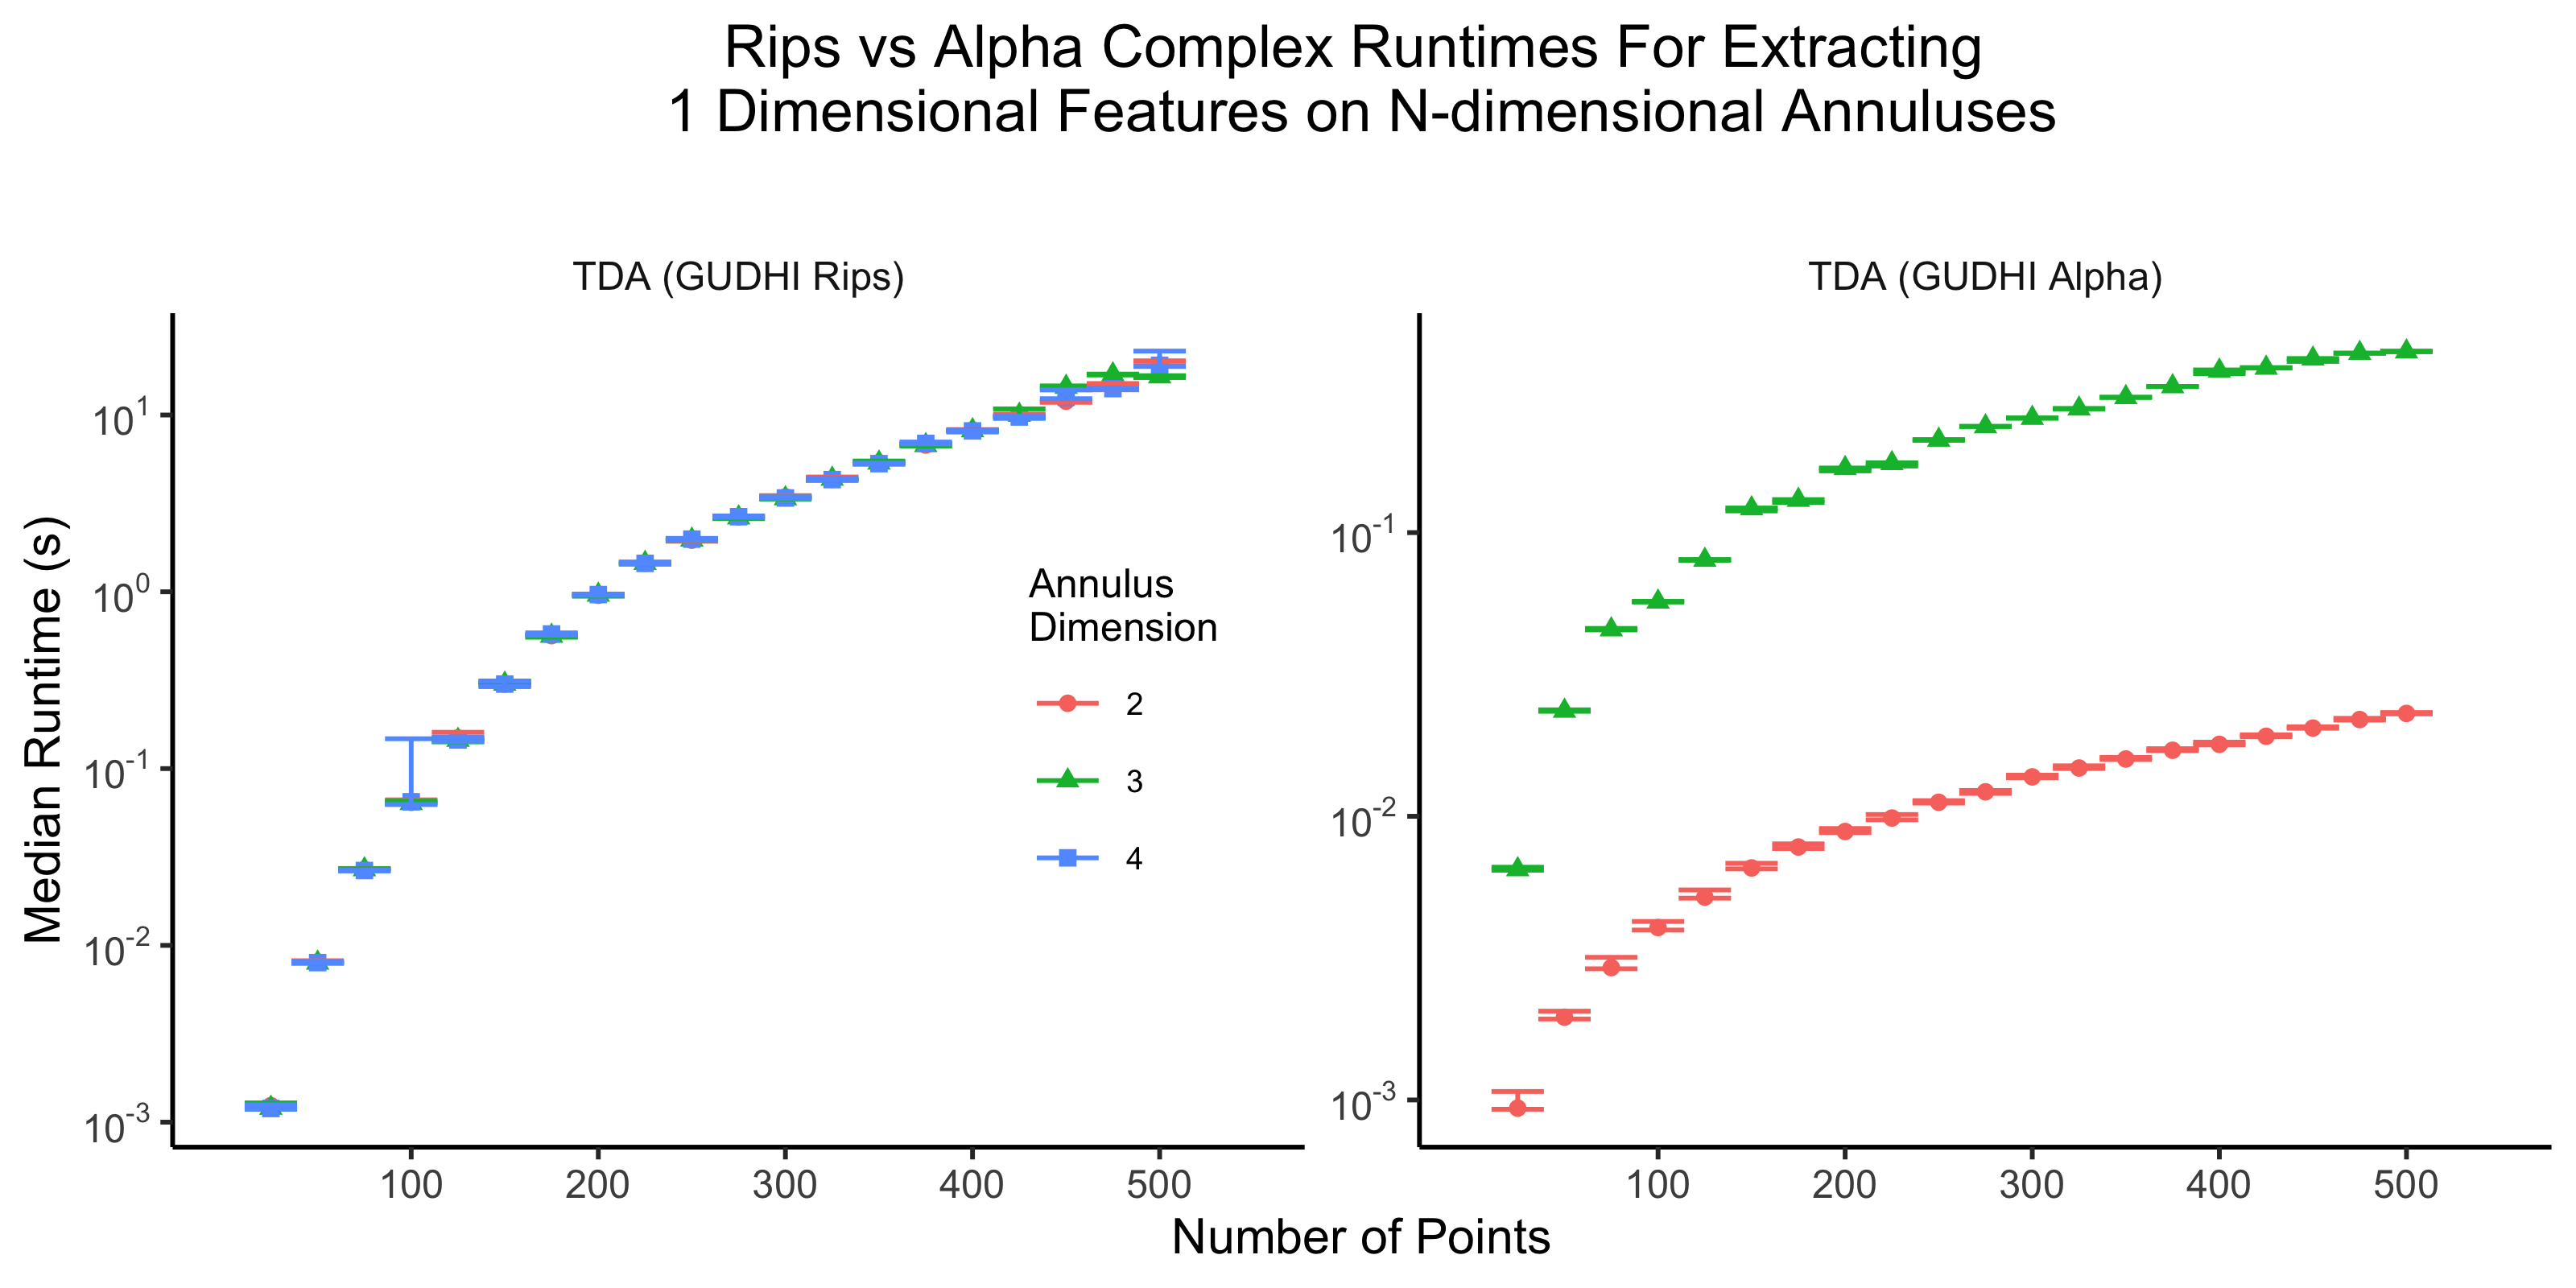
\includegraphics[width=6in]{fig6.png}
  \caption{
    \textbf{Comparing persistent homology calculation between Vietoris-Rips and alpha complices.}
    Median runtime (min to max, $n=10$ iterations per data point) for various data dimensions (denoted by color) are plotted against point cloud size and faceted by type of simplicial complex.
    Maximum of feature dimension was kept constant at 1.
    Alpha complex runtimes are linear, in contrast to polynomial Vietoris-Rips runtimes (see Supplement for regression details).}
\label{fig:ann}
\end{figure}

In addition to runtime differences, the three Vietoris-Rips homology
engines differ in memory use. All three engines appeared to follow power
law growth, with a linear trend on log-log plots (Figure \ref{fig:mem}).
However, for nearly all combinations of point cloud dimension and shape,
TDAstats used the least memory, and Dionysus used the most, with TDAstats
also growing with the smallest power law exponent as the number of
points increased for most point clouds. For most point clouds, runtime
and memory complexity for TDAstats (Ripser) grew with a power function
at least one degree less than the other engines (Figure \ref{fig:bigO}).

\begin{Schunk}
\begin{figure}
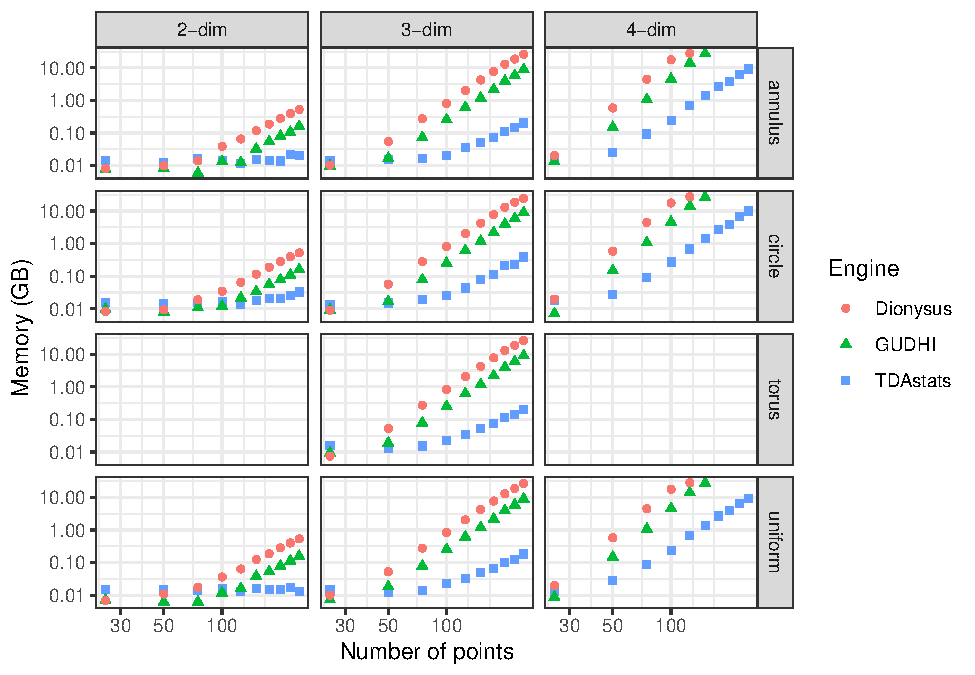
\includegraphics{fig7.pdf} \caption{\label{fig:mem}\textbf{Comparing memory use of Vietoris-Rips persistent homology engines.} Each column title corresponds to point cloud dimension; each row title lists point cloud shape; each persistent homology engine is represented by points of a distinct shape and color. For point clouds containing more than 50 points, there appears to be a linear trend on the log-log axes. Data for 2- and 4-dimensional tori were not collected because a torus does not trivially generalize to dimensions other than 3. Missing points for GUDHI and Dionysus in the 4-dim plots indicate that persistent homology calculation was terminated since memory requirement exceeded available RAM (32 GB).}\label{fig:memory}
\end{figure}
\end{Schunk}

\begin{Schunk}
\begin{figure}
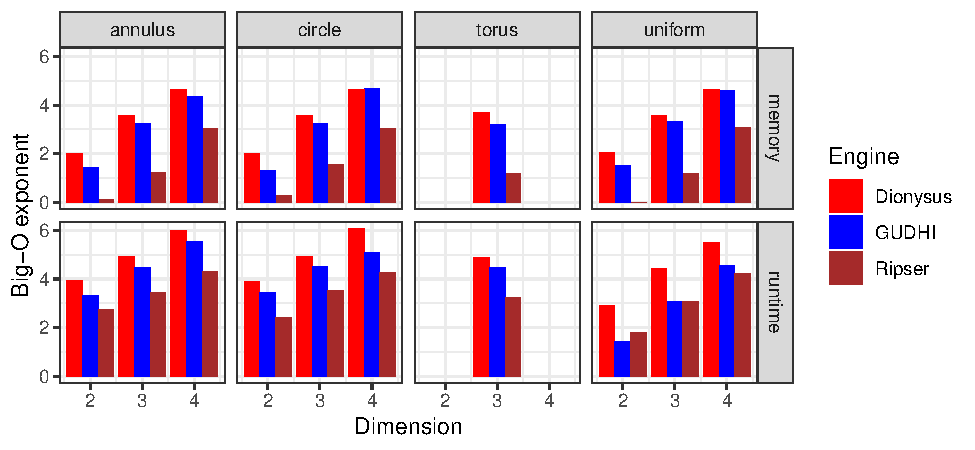
\includegraphics{fig8.pdf} \caption{\label{fig:bigO}\textbf{Big-O exponents for runtime and memory complexity as point cloud size varies.} In the majority of cases, Ripser (and consequently, TDAstats) has the lowest exponent, indicating the slowest growth in complexity as point cloud size increases. Due to shape constraints, torus only has data available in the third dimension.}\label{fig:bigoh}
\end{figure}
\end{Schunk}

\hypertarget{discussion}{%
\section{Discussion}\label{discussion}}

As persistent homology calculations continue to become a more popular
tool to analyze complex multidimensional data, it will be important to
understand from a computational perspective which method to use. In this
paper, we examined two forms of persistent homology complexes:
Vietoris-Rips and alpha complexes. Both algorithms describe topological
features through the generation of simplicial complexes. The advantage
in saving computational time by choosing a particular algorithm depends
on point cloud characteristics.

Figure \ref{fig:fin} shows that at high point cloud sizes, GUDHI's alpha
complex outperforms Ripser. Theoretically, alpha complexes gain
polynomial run time complexity as the number of points increases, whereas
Vietoris-Rips complexes gain exponential run time complexity
\citep{roadmap}. Specifically, alpha complexes are \(O(n^{d/2})\), and
Vietoris-Rips complexes are \(O(2^n)\), where \(n\) is the number of
points on a point cloud and \(d\) is the dimensions on the point cloud.
For the conditions in our paper, Vietoris-Rips and alpha complexes both
performed better than their theoretical maximums. Vietoris-Rips complex
calculations consistently had a polynomial growth for both runtime and
memory, while alpha complexes had linear runtime growth.

\begin{figure}
  \centering
  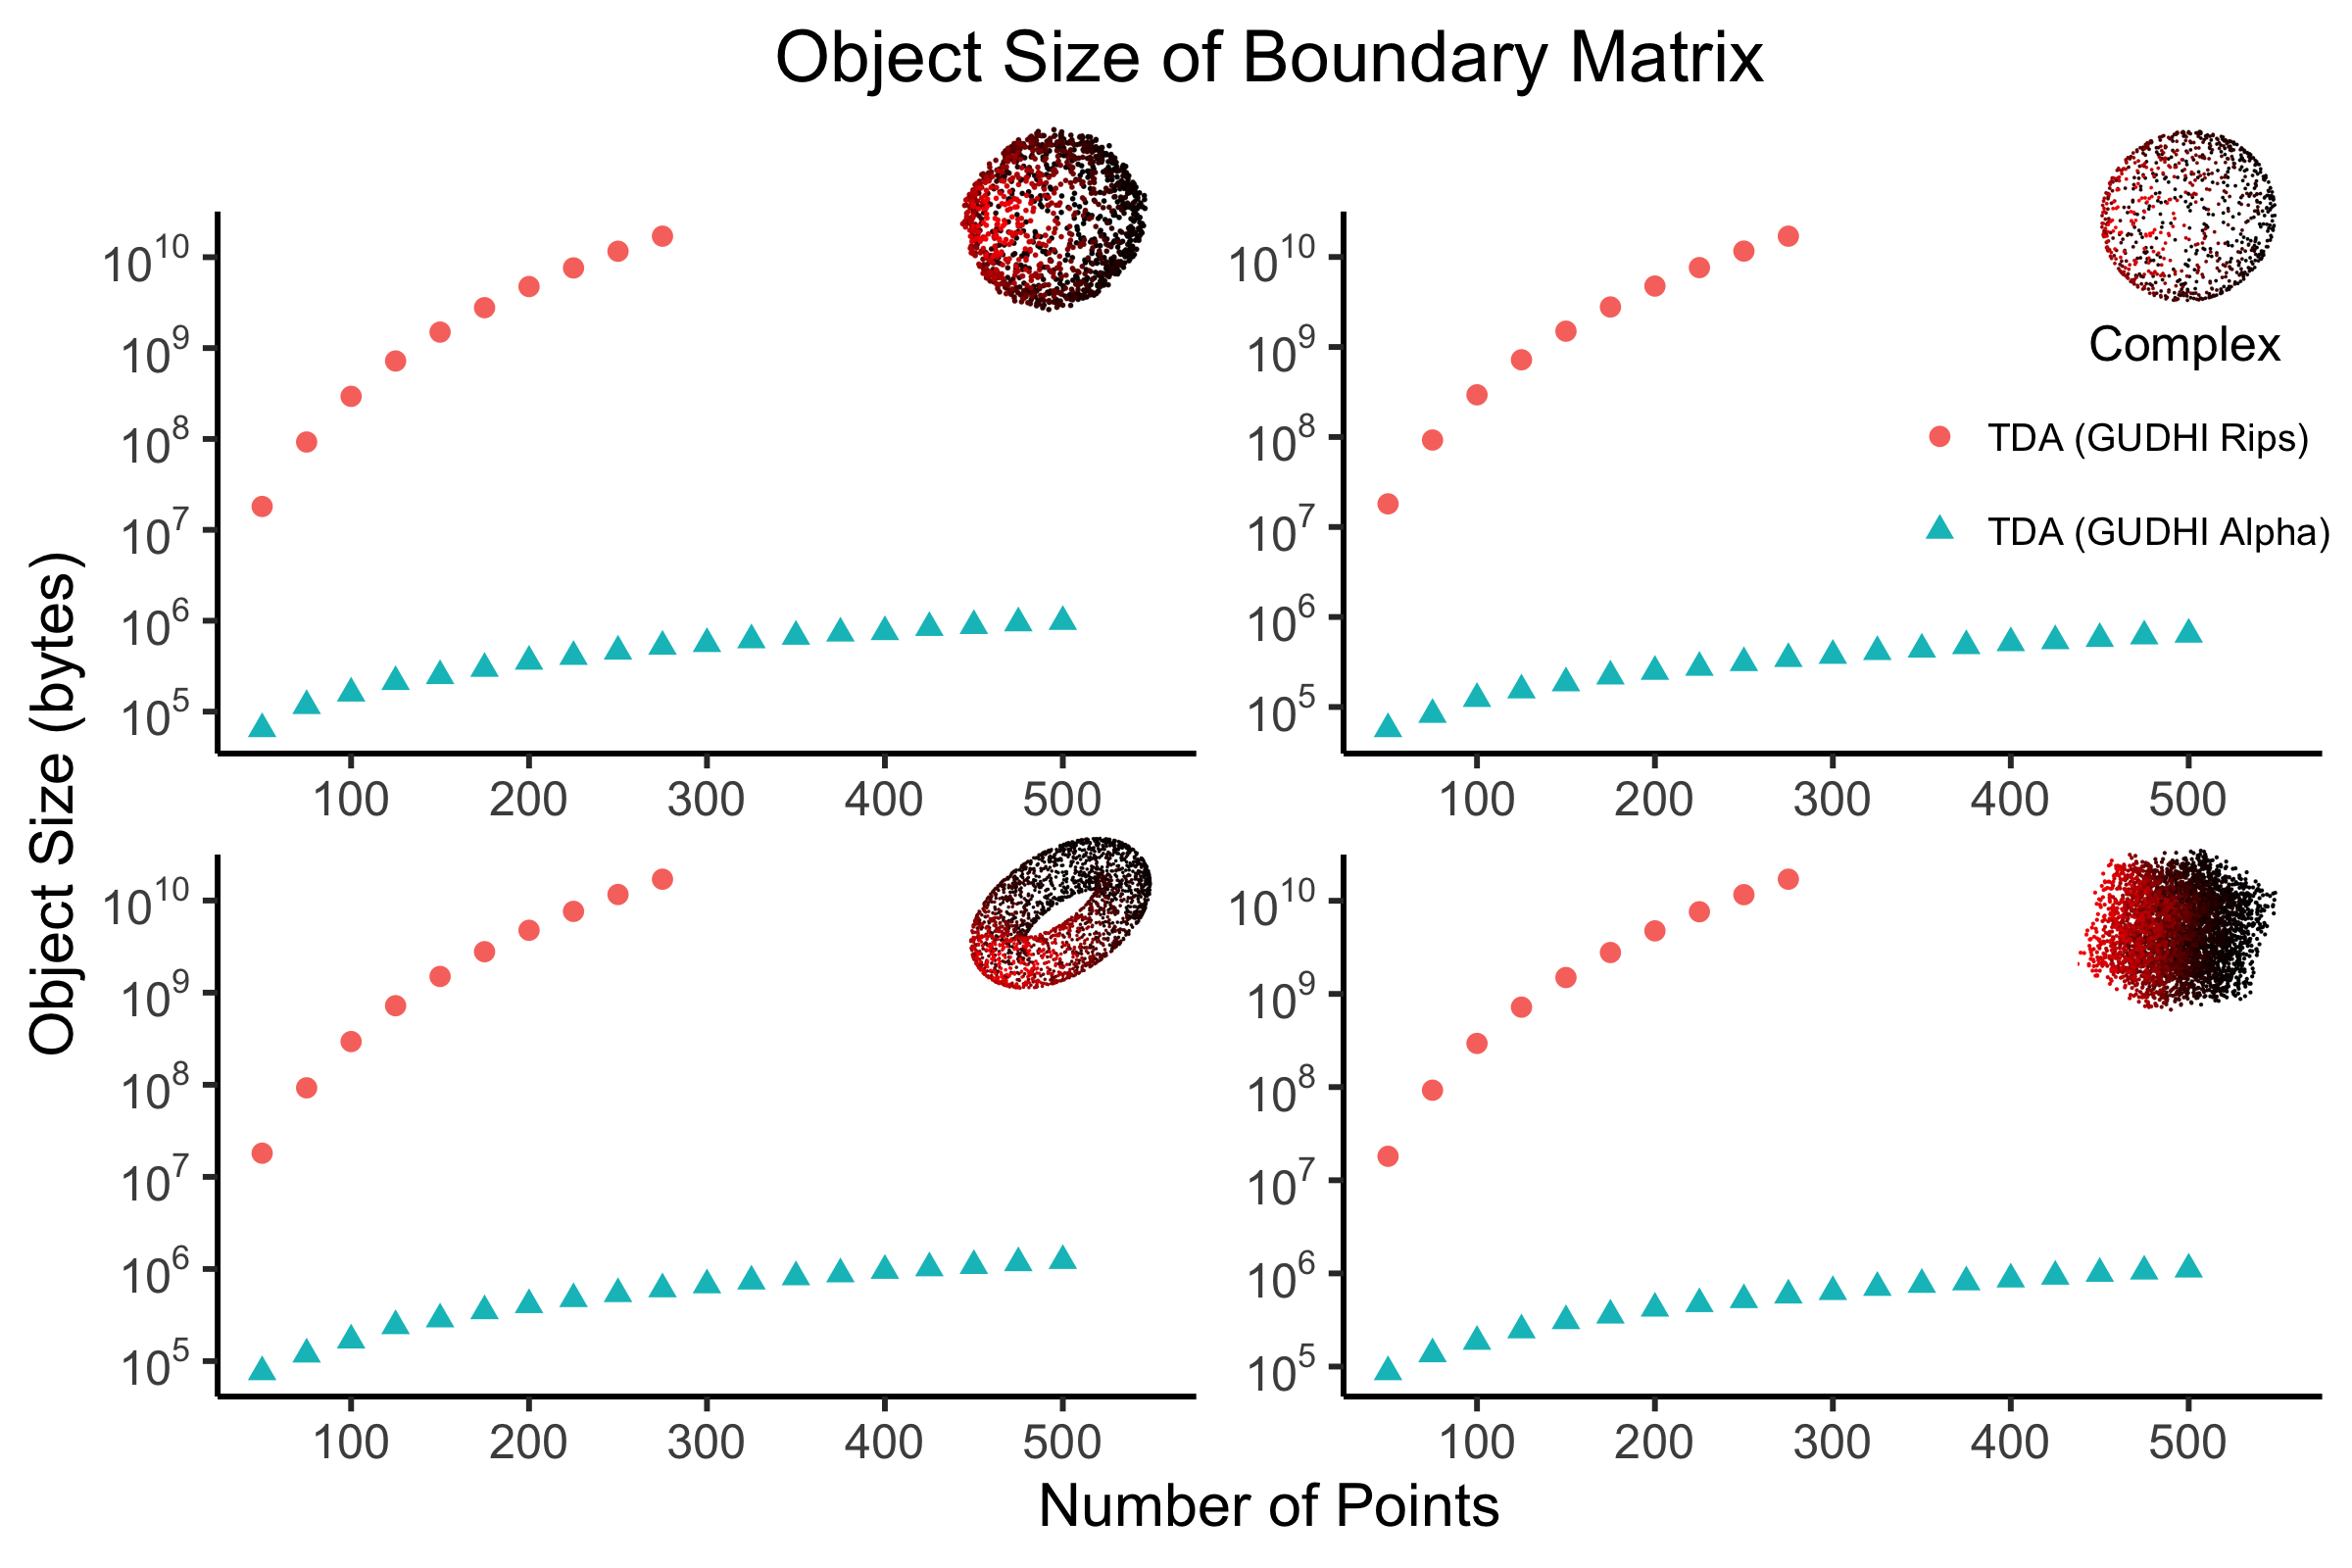
\includegraphics[width=6in]{fig9.png}
  \caption{
    \textbf{Runtime comparison of persistent homology calculation between Ripser's Vietoris-Rips and GUDHI's alpha complex functionality.}
    Median runtime (min to max $n=10$ iterations per data point) for various 3-dimensional point cloud structures (facet) plotted against point cloud size for each library (color).
    Benchmarking was conducted on an annulus (top-left), a sphere (top-right), a torus (bottom-left), and a cube (bottom-right).
    Data was not collected for data dimensions greater than 3 due to computational limitations of calculating alpha complices.}
\label{fig:fin}
\end{figure}

Based on the theoretical complexity and our results, alpha complexes are
superior for point clouds with 3 or fewer dimensions. This advantage
becomes especially clear at a high number of points. This difference in
performance is clear in both runtime and memory use. Interestingly,
while alpha complexes had overall less memory use, the memory use varied
depending on the shape. Alpha complexes seem to require more memory for
noisier data sets such as the annulus when compared to the sphere.

However, without sufficient computational resources, alpha complexes
were not usable for point cloud dimensions greater than 3. If a point
cloud has more than 3 dimensions, then it could undergo pre-processing
with dimension reduction before using alpha complexes. Note, it is
possible an algorithm will eventually be developed to enable alpha
complex computation of higher-dimensional data. However, if data
dimension cannot be reduced without significant information loss, then
Vietoris-Rips complexes should be used. It should be stated that if a
point cloud is compatible with both complexes, both analyses should be
performed as there may be a variation in the persistent homology matrix.
This is because alpha complexes satisfy the Nerve Theorem
\citep{alpha-complex}, which implies that they are topologically
equivalent to the true underlying topology of the dataset; in contrast,
Vietoris-Rips complexes only approximate the underlying topology
\citep{Rips-Complex}. Among the tested Vietoris-Rips engines, Ripser
(wrapped by \CRANpkg{TDAstats}) has the fastest calculation time. GUDHI
and Dionysus (wrapped by \CRANpkg{TDA}) significantly fall behind as
feature dimension and number of points increase.

On average, Ripser computed the persistent homology of a Vietoris-Rips
complex with less memory than either GUDHI or Dionysus. Thus, when
efficiency is critical, useRs would likely find \CRANpkg{TDAstats} the
appropriate library. However, \CRANpkg{TDA} contains an entire library
of features not available in \CRANpkg{TDAstats}. Specifically,
\CRANpkg{TDA} allows kNN density estimation, kernel density estimation,
density-based clustering, and dendrogram visualization, among other
useful functionality. When computational resources are plenty, when
point clouds are small and low-dimensional, or when the aforementioned
functionality is required, \CRANpkg{TDA} will likely be more appropriate
than \CRANpkg{TDAstats}. Both packages are hosted on CRAN.

While Vietoris-Rips complexes can handle high-dimensional data well, the calculation still significantly slows down when looking for higher
dimension features. This is evidenced by the big-O polynomial growth for
runtime and memory that have degree less than 4 for most 2-dimensional
point clouds, but degree between 4 and 6 for most 4-dimensional point
clouds (Figure \ref{fig:bigO}); even higher degree complexities should
be expected as point cloud dimension increases. Thus, finding
high-dimensional topological features in high-dimensional point clouds
remains a challenge. Methods to calculate persistent homology do exist
for other simplicial complexes, such as the Delaunay complex and the
Witness complex, but, to our knowledge, they are not currently
implemented in CRAN packages. Future challenges would be creating and
implementing algorithms that reduce the computational complexity of
higher-dimensional topological feature calculations for R.

\hypertarget{acknowledgments}{%
\section{Acknowledgments}\label{acknowledgments}}

The authors thank Emily Dolson, PhD for assistance with using a
high-performance computing node for data collection. JGS was supported
by NIH grant R37 CA244613.

\bibliography{wadhwa-tda}


\address{%
Eashwar V. Somasundaram\\
School of Medicine\\%
Case Western Reserve University\\ Cleveland, OH 44106, United States\\
%
%
%
\\\href{mailto:eashwar.somasundaram@case.edu}{\nolinkurl{eashwar.somasundaram@case.edu}}
}

\address{%
Shael E. Brown\\
Department of Quantitative Life Sciences\\%
McGill University\\ Montreal, QC H3A 0G4, Canada\\
%
%
%
\\\href{mailto:shael.brown@mail.mcgill.ca}{\nolinkurl{shael.brown@mail.mcgill.ca}}
}

\address{%
Adam Litzler\\
Department of Translational Hematology and Oncology Research\\%
Cleveland Clinic Foundation\\ Cleveland, OH 44195, United States\\
%
%
%
\\\href{mailto:adli4611@colorado.edu}{\nolinkurl{adli4611@colorado.edu}}
}

\address{%
Jacob G. Scott\\
Department of Translational Hematology and Oncology Research\\%
Cleveland Clinic Foundation\\ Cleveland, OH 44195, United States\\
%
%
%
\\\href{mailto:ScottJ10@ccf.org}{\nolinkurl{ScottJ10@ccf.org}}
}

\address{%
Raoul R. Wadhwa\\
Cleveland Clinic Lerner College of Medicine\\%
Case Western Reserve University\\ Cleveland, OH 44195, United States\\
%
%
%
\\\href{mailto:raoul.wadhwa@case.edu}{\nolinkurl{raoul.wadhwa@case.edu}}
}

